\documentclass{NSF}
\usepackage{amssymb}
\usepackage{amsmath}
\usepackage{graphicx}
\usepackage[table,xcdraw]{xcolor}
\graphicspath{ {images/} }


\begin{document}
\author{Myunggun Seo,  Guyu Fan, and Nischal Mainali \\ Professor: Saurabh Ray}
\date{December 15, 2018}
\title{
  {\normalfont Computer Science Capstone Progress Report} \\ 
  Lifting Squares to a Half-space: a Specific Case of Lifting Pseudo-disks
}
{\let\newpage\relax\maketitle}

\section{Abstract}
% Your short version of your proposal goes here
A half-space in $\mathbb{R}^3$ is either of the two parts separated by a plane. Because of some helpful properties that exist in half-spaces, it is often useful to map geometries in a plane to half-spaces in  $\mathbb{R}^3$. In this project, we attempt to prove or disprove the existence of a mapping from a family of squares in a plane to a family of half-spaces in $\mathbb{R}^3$ such that all points inside each square are mapped to points inside the corresponding half-space and all points outside each square are mapped to points outside the corresponding half-space. If such a mapping can be shown to exist, we attempt to provide a mathematical description of it or find an algorithm that performs the mapping. \cite{mainali2018}
\tableofcontents

\section{Introduction}
\subsection{General Case of Lifting Pseudo-disks}
The problem that we tackle is a specific case of an unsolved problem in computational geometry: 

Given a set of pseudo-disks $\{D_i\}$ and points $\{P_j\}$ in $\mathbb{R}^2$ in arbitrary positions, (1) determine the existence of a mapping and (2) describe the mapping from the pseudo-disks and points to a set of half-spaces $\{H_i\}$ and points $\{Q_j\}$ in $\mathbb{R}^3$ such that the membership of point $P_j$ in a pseudo-disk $D_i$ is preserved with point $Q_j$ in $H_i$. 

Because shapes in $\mathbb{R}^2$ are mapped to a higher dimension $\mathbb{R}^3$, we will call this problem "lifting." Note that lifting a pseudo-disk to a half-space does not require that the entire half-space to be occupied, but only that no point in the half-space is lifted from the exterior of the pseudo-disk.

Lifting is part of a class of mapping methods in Combinatorial Geometry which proved useful because such a map provides another representation and thus new properties to a geometric configuration. Such new properties are used often in cases such as finding lower bounds on $\epsilon$-nets or in Kernel Trick in Machine Learning. 

Although there are specific cases of pseudo-disks such as circles (?) (and anything else? ovals? parabolas? all conic sections?) where this mapping exist and described algebraically, it is not known whether there is such a mapping for other seemingly simple cases like rectangles or squares. 

\subsection{Case of Squares of Equal Size}
Problem statement: Given a set of squares of  $\{S_i\}$ and points $\{P_j\}$ in $\mathbb{R}^2$ in arbitrary positions, is there a mapping from the squares and points to a set of half-spaces $\{H_i\}$ and points $\{Q_j\}$ in $R^3$ such that the membership of point $P_j$ in a square $S_i$ is preserved with point $Q_j$ in $H_i$? If there is, what is the mapping? 

\section{Problems Related to Pseudo-disk Lifting Problem}
\subsection{Solution: Lifting an interval}
This is the lowest abstraction of a pseudo-disk that we consider. An interval in $\mathbb{R}$ can be considered both as a circle (or ball) and a square (or $k$-cell). The interval, using the definition of a ball, defined as $|x-a|\leq r$ is equivalent to $(x-a)^2 \leq r^2$ and $x^2-r^2$ is substituted with $y$ to construct the half-space in $\mathbb{R}^2$: $-2ax+y+a^2 \leq 0$.  Point $x=\alpha$ is lifted to $(\alpha, \alpha^2)$. Then all points inside the original interval of length $2r$ becomes placed underneath the hyperplane in $\mathbb{R}^2$ which is a line.
\begin{align*}
\alpha & \mapsto (\alpha,\alpha^2) \\
|x-a|\leq r & \mapsto -2ax + y + a^2 \leq 0
\end{align*}


\subsection{Solution: Lifting disks of equal radii}
\begin{figure}[ht]
\centering
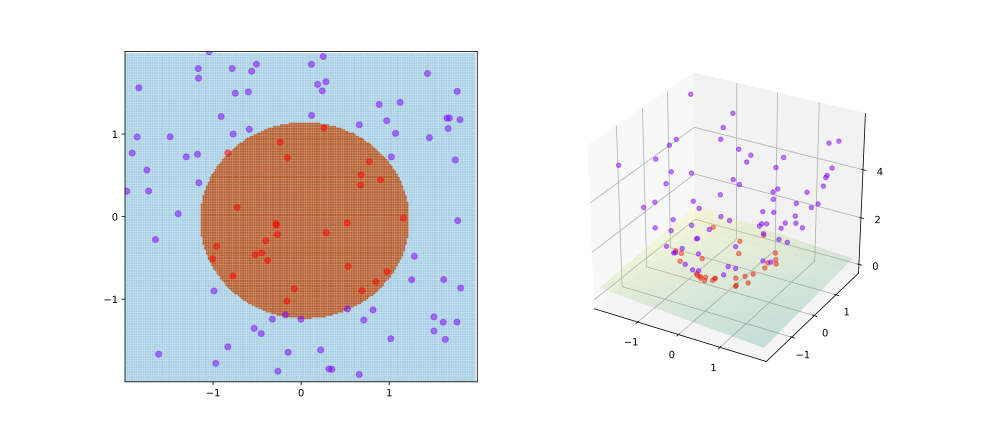
\includegraphics[width=\textwidth]{kernel-trick}
\caption{Red points inside a single disk in $\mathbb{R}^2$ are mapped to a half-space in $\mathbb{R}^3$, allowing linear separation of points.  (Source: Wikipedia - Kernel Method) }
\end{figure}

There is an algebraic lifting from disks to half-spaces. Point $(\alpha,\beta)$ is lifted to $(\alpha,\beta,\alpha^2+\beta^2-r^2)$, and disk $(x-a)^2+(y-b)^2\leq r^2$ is lifted to $-2ax -2by + z + (a^2+b^2) \leq 0$ by substituting  $x^2+y^2-r^2$ with $z$. 
\begin{align*}
(\alpha,\beta) & \mapsto (\alpha,\beta,\alpha^2+\beta^2-r^2) \\
(x-a)^2+(y-b)^2\leq r^2 & \mapsto -2ax -2by + z + (a^2+b^2) \leq 0
\end{align*}

The limitation of this method is that it is only possible for disks of equal radii since all points in $\mathbb{R}^2$ can only map to the same point in $\mathbb{R}^3$ which will be defined by the radius $r$.

\subsection{Solution: Lifting disks of varying radii}
Using a similar approach as the above problem, Point $(\alpha,\beta)$ is lifted to $(\alpha,\beta,\alpha^2+\beta^2)$, and disk $(x-a)^2+(y-b)^2\leq r^2$ is lifted to $-2ax -2by + z + (a^2+b^2-r^2) \leq 0$ by substituting  $x^2+y^2$ with $z$. 
\begin{align*}
(\alpha,\beta) & \mapsto (\alpha,\beta,\alpha^2+\beta^2) \\
(x-a)^2+(y-b)^2\leq r^2 & \mapsto -2ax -2by + z + (a^2+b^2-r^2) \leq 0
\end{align*}

\subsection{Idea: Straightening pseudo-disks to disks}
If there is a way to "straighten," or map, a set of general pseudo-disks to disks, then there must be a way to lift any pseudo-disk to a half-space by straightening the pseudo-disks to disks and lifting the produced disks.

\subsection{Idea: Straightening pseudo-lines to lines}
A similar problem to straightening pseudo-disks to disks is straightening pseudo-lines. Pseudo-lines are a set of curves that intersect one another at most once. This property derives from that of lines. The problem statement is:  given a set of $n$ pseudo-lines, find a positioning of $n$ lines so that the vertical order of the lines match that of the pseudo-lines. This is not always possible to do. (? counter example?)




\subsection{Idea: Lifting pseudo-disks to a polytope}
We can see a pseudo-disk as an (infinite) intersection and complements of circles of varying radii. Assuming we can lift disks of varying radii to $\mathbb{R}^3$, the geometry lifted to $\mathbb{R}^3$  from a pseudo-disk can be seen as the intersection and complements of each half-space resulting from lifting the subordinate circles. However, the limitation of this method is that it does not produce half-spaces but produces polytopes which may or may not be convex.




\section{Problems Related to Square Lifting Problem}

\subsection{Case of lifting axis-parallel non-piercing rectangles}
For any pair of axis-parallel non-piercing rectangles, there exist three cases of their positioning:
\begin{enumerate}
\item two disjoint rectangles, without any intersections
\item one rectangle has two corners of the other rectangle inside it
\item each rectangle has a corner in the interior of each other
\item (?) one is completely inside the other
\end{enumerate}
Rectangles are defined by two inequalities ($a\leq x \leq b$ and $c \leq y \leq d$ which is one more than what defines a half-space so it is impossible?

\subsection{Solution for lifting rectangles that are fixed to the $x$,$y$-axes}
These rectangles are hinged at the origin. For positive $a,b$ values, a rectangle are defined by two inequalities: 
\begin{equation}\label{origin-hinged-1}
0 \leq x \leq a,\  0\leq \  y \leq b
\end{equation}
Since a half-space is defined by just one inequality, we would like to combine the two inequalities into one: 
\begin{equation}\label{origin-hinged-2}
\frac{x}{a} + \frac{y}{b} \leq 2
\end{equation}
Now, \eqref{origin-hinged-1} implies \eqref{origin-hinged-2} but \eqref{origin-hinged-2}  may not imply \eqref{origin-hinged-1}. For \eqref{origin-hinged-2} to imply \eqref{origin-hinged-1}, the values of $x$ and $y$ must satisfy the following: if either $\frac{x}{a}$ or $\frac{y}{b}$ is greater than 1, it should be greater than 2. This means that if $\frac{x}{a}+\frac{y}{b}$  is less than 2, both of its terms are less than 1.

We fulfill the requirement by applying "exponential stretching" on the given set of finite points and rectangles in both $x$ and $y$ directions so that $\frac{x}{a} \geq 2$  for points of which the $x$ coordinate lies beyond the line $x=a$ and $\frac{y}{b} \geq 2$ for points of which the y coordinate lies beyond the line $y=b$. 

Then, the inequality \eqref{origin-hinged-2} represents a half-space in $\mathbb{R}^3$. This solution provides a minimum bound on the feasibility of lifting squares or rectangles in general.



\subsection{Solution for lifting rectangles that are fixed to the $x$-axis}
\paragraph{Approach 1}
In order to update the minimum bound, consider a finite set of points and rectangles in the first quadrant of $\mathbb{R}^2$, each type of which are defined by the constraints

\begin{align*}
    \text{point:}& \ x \in \mathbb{R},\  z \geq 0 \\
    \text{rectangle:}& \ x_i \leq x \leq x_j,\ 0 \leq z \leq c
\end{align*}

We refer to such rectangles as "buildings," and the two lines $x=x_i$ and $x=x_j$ "walls."
We would like to combine the three constraints of the rectangle as a single inequality representing a half-space in $\mathbb{R}^3$.
Using ideas from exponential stretching, first sort the $x$ coordinates of all points and all walls together and incrementally assign an integer index to each of them. Stretch out the coordinates of points and walls along the $x$-axis using a steep convex function such as $f(x)=2^x$. 
(? how steep should it be? so that lij(xk) > delta if xk not in building? this would be to force lij to exceed 0 by a lot if it exceeds at all)
The $i$th $x$ coordinate, be it of a point or a wall, will be mapped to a point in $\mathbb{R}^2$
\begin{equation}
	x_i \mapsto (i, f(i))
\end{equation}
so that if $x_k \in [x_i,x_j]$(ie. the $k$th point is within the walls $x_i,x_j$ of a building), then $l_{ij}(x_k) \leq 0 $, where $l_{ij}$ for the rectangle with walls  $i$th and $j$th vertical lines is defined as

\begin{equation*}
    l_{ij}(x_k) = [f(k) - f(i)] -[\frac{f(j)-f(i)}{j-i}(k - i)]
\end{equation*}


We need steep functions because we want to maximize $l_{ij}$ when $x_k$ is not between $x_i$ and $x_j$.
A building's two constraints are respectively changed to 

\begin{equation}\label{x-axis-hinged-separate}
    l_{ij}(x) \leq 0, \ \frac{z}{c} \leq 1
\end{equation}


We need to combine these two inequalities into a single inequality that defines a half-space in $\mathbb{R}^3$. 
The two constraints in \eqref{x-axis-hinged-separate} imply the following inequality:
\begin{equation}\label{x-axis-hinged-added}
    l_{ij}(x) + \frac{z}{c} \leq 1 
\end{equation}
To make the converse true, we must have that if $l_{ij}(x)$ exceeds 0, it exceeds 1. $\epsilon$ is the smallest magnitude that $l_{ij}$ can have for the given set of points when $x$ is outside $x_i$ and $x_j$ so that the first term becomes greater than 1 if it's violated. $\delta$ is the greatest magnitude of all $l_{ij}$'s for when $x$ is outside $x_i$ and $x_j$. Then we should exponentially stretch in $z$ direction as well so that when the first term is negative but $\frac{z}{c}$ is greater than 1, it compensates for the negative term. The stretching in $z$ direction should satisfy $\frac{z}{c} \geq 1+\frac{\delta}{\epsilon}$.
\begin{equation}
	\frac{l_{ij}(x,y)}{\epsilon} + \frac{z}{c} \leq 1
\end{equation}
\paragraph{Approach 2}
Another approach to lift a set of buildings is by fitting circles on them. Stretch the buildings horizontally so that the ratio between the maximum height of the buildings and the maximum width of the buildings is minimal. For each of the buildings, fit an arc around it. This is possible and conserves point memberships. The arcs are part of a larger disk and we achieve our goal by lifting those disks.

\section{Mapping squares to disks}
It would be enough to find a mapping from a square to disks that preserves point memberships to show that squares can be lifted to half-spaces. Since lifting disks of varying centers and is possible, squares can be lifted via mapping squares to disks and then lifting the disks to half-spaces.

In fact, since we already know that disks can be lifted to half-spaces, the statement that squares or rectangles can be mapped to disks is a stronger statement than the statement that squares or rectangles can be lifted to half-spaces. 

First, we try to find which intersection patterns are impossible to create with disks while they may be possible for other pseudo-disks, namely squares.

\subsection{Squares in star formation}

\begin{figure}[ht]
\centering
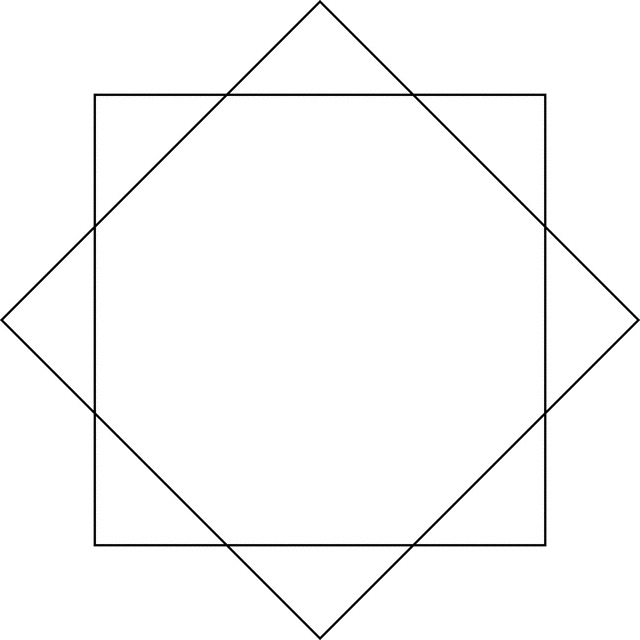
\includegraphics[width=\textwidth,height=5cm,keepaspectratio]{cocentric-squares}
\caption{ A pair of disks cannot have exactly 8 intersections and 10 regions  defined by them }
\end{figure}

Considering squares of various radii, positions, and tilt, it is easy to show that it is impossible to map squares in general to disks while preserving point memberships. For instance, take two co-centric squares of equal size but at a 45 degree angle of each other. This configuration produces a total of 8 intersections and 10 regions. No pair of circles in a plane can produce 10 regions and thus general squares cannot be mapped to disks.

\subsection{Pattern of all k-depth regions for k=0,1,2 }
It is impossible lay out $n$ circles to include all combinatorially possible regions of $depth=2$ for $n \geq 5$. This can be demonstrated by constructing a graph with vertices representing each disk and an edge connecting two vertices if the corresponding disks share a common $depth=2$ region. Creating all combinatorially possible regions of $depth=2$ means each vertex is connected to all other vertices -- in other words it is a complete graph. For $n \leq 4$, it is possible to draw a planar complete graph but for $n \geq 5$ it is impossible to draw a planar complete graph.

It is important to note, however, there is  a limit to the number of $depth=2$ regions that can be created by axis-parallel rectangles. 

\section{Mapping disks to squares}
We approach the above case from the inverse mapping. If there is a mapping from disks to squares, we might be able to utilize the mapping to construct a mapping from squares to disks. This begs the question: can we draw an arrangement of pseudo-disks/pseudo-disks/disks/disks that cannot be converted into disks/rectangles/rectangles/squares? The two approaches below explain that some configurations of circles are not represented in any configuration of axis-parallel squares.

\paragraph{Approach 1} The following is an incomplete proof that it is impossible to map disks to squares:
For three disks, there can be maximum three $depth=2$ regions. Every time we add another disk, three more are formed, amounting to $3n-6$ regions of $depth=2$   for $n$ disks. 
For squares, the seemingly greedy number of $depth=2$  regions newly formed by adding a new square is 2 and so the total number of $depth=2$ regions is $2n$.
Since $3n-6 > 2n$ for all $n > 6$, a family of 7 or more disks has regions represented that are not reproducible with a family of equal number of axis-parallel squares.

This proof is incomplete because it is not certain that $2n$ is the optimal number of $depth=2$ regions for the maximum number of $n$ squares.

\paragraph{Approach 2} Guyu's bump argument
Consider a depth=3 region created by intersections of squares. The region is rectangular in shape. At least two of its four neighbours (up, down, left, right) must have depth=2. (?why?)

\paragraph{Approach 3} Multiple ($n\geq3$) circles sharing one intersection point.


\section{Reducing counterexamples of unrepresentable half-spaces}
Hypothetically, computers can check all combinations (with 5 squares there are already 16 possible regions) to claim that a certain configurations of squares and points can topologically map or not. If it's not possible to map a certain configuration of squares and points, there would be a logical inconsistency in the system somewhere. Instead of checking all combinations, it would be ideal to check a smaller number of combinations  to conclude that a mapping is impossible. Thus it would be helpful to show that any counterexample can be reduced to a small counterexample, say of size two or three squares.

We approach this problem from a lower level, using pseudo-lines in $\mathbb{R}^2$ instead of half-spaces in $\mathbb{R}^3$. A matrix is used to abstractly describe the configuration of the pseudo-lines and points on the plane. Each row of the matrix represents a pseudo-line $c_i$ and each column represents a point $p_j$. 
\begin{equation*}
M_{ij} =\begin{cases}
            	+1 & \text{if $c_i$ is above $p_j$,} \\
                -1 & \text{if $c_i$ is below $p_j$}
            \end{cases}
\end{equation*}
Without loss of generality, choose the following as the "forbidden pattern:" 
\begin{equation}
\begin{bmatrix}
    +1 & -1 \\
    -1 & +1 
\end{bmatrix}
\end{equation}
The above pattern appears whenever an inconsistency exists in a system of two or more curves and three or more points:
\begin{align*}
\begin{bmatrix}
    +1 & -1 & +1 \\
    -1 & +1 & -1
\end{bmatrix} \text{ or }\ 
\begin{bmatrix}
    -1 & +1 & -1  \\
    +1 & -1 & +1
\end{bmatrix}
\end{align*}
The two cases above cannot exist since pseudo-lines can only intersect each other at most once but these configurations necessarily mean that there are at least two intersections between the two curves. 

\subsection{No permutation of geometries}
Define a graph of vertices representing the pseudo-lines and a directed edge from $c_i$ to $c_j$ if for $a<b$ the following "intersection" pattern exists:
\begin{align*}
\centering
\begin{tabular}{l|lllll}
                      & p_a & \dots & p_b\\ \hline
c_i                  &  -1   &        &     +1   \\
\vdots          &            &         &           \\
c_j                  &   +1    &        &    -1
  \end{tabular}
\end{align*}
The existence of this pattern means that $c_i$ and $c_j$ intersect between the two points $p_a$ and $p_b$. Here we show that if there is a cycle of size $n$, it will inevitably admit the forbidden pattern. Suppose there exists a cycle of size $n$ without any forbidden patterns:
\begin{align*}
\centering
\begin{tabular}{l|lllll}
                      & \dots & 2n-3 & 2n-2 & 2n-1 & 2n \\ \hline
c_1              &            &        &          &  +1    &  -1   \\
\vdots          &            &         &          &          &    \\
c_{n-1}   &            &  -1    &  +1    &          &    \\
c_{n}      &             &  +1   &   -1  &  -1    &  +1 
  \end{tabular}
\end{align*}

Since this matrix does not have any forbidden patterns, $c_1$ must be above $p_{2n-3}$.
\begin{align*}
\centering
\begin{tabular}{l|lllll}
                      & \dots & 2n-3 & 2n-2 & 2n-1 & 2n \\ \hline
c_1              &            & \cellcolor[HTML]{FFFFC7}{\color{blue}+1}       &          & \cellcolor[HTML]{FFFFC7} +1    & -1    \\
\vdots          &            &         &          &          &    \\
c_{n-1}   &            &  -1    &  +1    &          &    \\
c_{n}      &             & \cellcolor[HTML]{FFFFC7} +1   &   -1  &\cellcolor[HTML]{FFFFC7}  -1    &  +1 
\end{tabular}
\end{align*}
Since this matrix does not have any forbidden patterns, $c_{n-1}$ must be above $p_{2n}$.
\begin{align*}
\begin{tabular}{l|lllll}
                      & \dots & 2n-3 & 2n-2 & 2n-1 & 2n \\ \hline
c_1              &            &\cellcolor[HTML]{FFFFC7} +1       &          &  +1    &\cellcolor[HTML]{FFFFC7} -1    \\
\vdots          &            &         &          &          &    \\
c_{n-1}   &            &  \cellcolor[HTML]{FFFFC7}-1    &  +1    &          &  \cellcolor[HTML]{FFFFC7} {\color{blue}-1} \\
c_{n}      &             &  +1   &   -1  &  -1    &  +1 
\end{tabular}
\end{align*}
However, we have a contradiction since there exists a forbidden pattern:
\begin{align*}
\begin{tabular}{l|lllll}
                      & \dots & 2n-3 & 2n-2 & 2n-1 & 2n \\ \hline
c_1              &            & +1       &          &  +1    & -1    \\
\vdots          &            &         &          &          &    \\
c_{n-1}   &            &  -1    & \cellcolor[HTML]{CB0000} +1    &          &  \cellcolor[HTML]{CB0000} -1 \\
c_{n}      &             &  +1   &  \cellcolor[HTML]{CB0000} -1  &  -1    & \cellcolor[HTML]{CB0000} +1 
\end{tabular}
\end{align*}
Thus if in a configuration of pseudo-disks there exists a cycle of size $\geq 3$, it must admit a small counterexample that is namely the forbidden pattern. This means that all that is needed to show that a system of pseudo-lines and points is inconsistent is to look for a single forbidden pattern.

\subsection{Permutable curves}

Define $-1 < +1$ and lexicographically sort all of the rows. If the forbidden pattern exists in the the sorted matrix, we know that there must be a cycle of size $\geq 3$.

\subsection{Permutable curves and points}

\subsection{Using Helly}

\section{Computational approach using Convex Optimization software}
We attempt using a convex optimization problem solver software in order to find a counterexample for a large number of points and squares. 

If for each execution the software finds a viable mapping from finite squares and points to half-spaces, it is inconclusive and does not imply anything. However, if the software concludes that there exist no mapping for a certain configuration of squares and points, such a configuration is the counterexample demonstrating that squares cannot be lifted to half-spaces in general. In either case, it could provide us with more insight on cases that are too big to be imaginable.

Below is the setup of the convex optimization problem. The idea is to create variables that represent points and half-spaces in $\mathbb{R}^3$. If a corresponding mapping from a given set of squares to half-spaces exist, the software will find it.

\begin{enumerate}
\item Randomly sample set of $m$ points in $\mathbb{R}^2$ \begin{equation*}
				P_i = (\alpha, \beta)
\end{equation*}
\item Randomly sample $n \times 4$ values that define $n$ axis-parallel squares \begin{equation*}
				S_j=(left,right,top,bottom)
			\end{equation*}
\item For each $i,j$ pair, save the binary membership flag \begin{equation*}
M_{ij} =\begin{cases}
            	1 & \text{if $P_i$ inside $S_j$,} \\
                -1 & \text{otherwise}
            \end{cases}
\end{equation*}
\item Create $m \times 3$ variables representing points in $\mathbb{R}^3 $ \begin{equation*}
			Q_i = (x_i,y_i,z_i, 1)
\end{equation*}
\item Create $n \times 3$ variables representing half-spaces in $\mathbb{R}^3 $ \begin{equation*}
				H_j = (a_j,b_j,c_j, 1)
\end{equation*}
\item Create $m \times n$ constraints \begin{equation*}
			M_{ij}(Q_i \dot H_j) > 0
\end{equation*}
\item Set the objective function as simple expression, say 1, and solve.

\end{enumerate}



\section{Appendix: Definitions}
\begin{enumerate}
\item A geometric shape is \textbf{axis-parallel} if it is parallel or aligned with a coordinate axis.
\item A \textbf{half-space} in $\mathbb{R}^3$ is either of the two parts separated by a plane. In general, a half-space is either of the two parts divided by a hyperplane in a $\mathbb{R}^k$.
\item \textbf{Helly's theorem} for the Euclidean plane states that if a family of convex sets has a nonempty intersection for every triple of sets, then the whole family has a nonempty intersection. (Wikipedia)
\item A \textbf{Jordan Curve} is a curve in a plane that is topologically equivalent to a disk - simple and closed.
\item \textbf{Lifting} is mapping a geometric shape in one dimension to a higher dimension.
\item \textbf{Membership} of a point and a region is a binary flag that signifies whether the point is inside the region or not.
\item A Jordan curve $C$ \textbf{pierces} another Jordan curve $D$ if all curves in the interior of $D$ connecting any two points inside $D$ must cross $C$ at least twice.
\item \textbf{Pseudo-disks} are a set of regions defined by the interior of Jordan curves in $\mathbb{R}^2$ in which any pair of the Jordan curves intersect at maximum two places and do not pierce one another. This property is derived from disks in $\mathbb{R}^2$. (?) Can they be inside one another?
\item \textbf{Pseudo-lines} are a set of curves that intersect one another at most once. This property derives from that of lines.
\item The \textbf{depth} of a region formed by the intersection of multiple Jordan curves is the number of Jordan curves that the region is inside of.

\end{enumerate}



\renewcommand\refname{References}
\bibliography{references}
% The IEEE bibliography style is NOT rBibliography listing all cited references.
% Feel free to use whatever style you prefer
\bibliographystyle{IEEEtran}

\end{document}

